\adparagraph{Adjusted nDCG}
In Figure \ref{fig:andcg} we see the scores of the adjusted nDCG measure. All methods generally have high levels of satisfaction according to the measure, with none scoring below 95 percent satisfaction.
This could point to some difficulties in measuring satisfaction with live data.

\begin{figure}[H]
	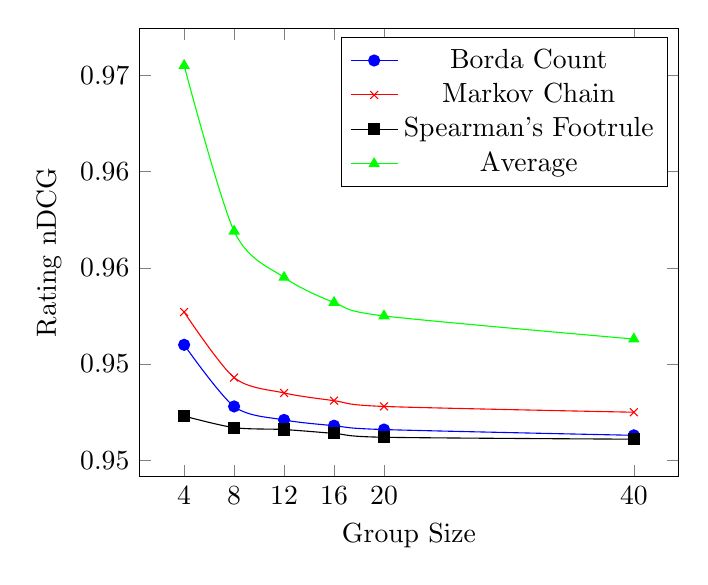
\begin{tikzpicture}
	\begin{axis}[
	xlabel=Group Size,
	ylabel=Rating nDCG,
	xtick = {4,8,12,16,20,40}]
	\addplot[smooth,mark=*,blue] plot coordinates {
		(4,0.956)
		(8,0.9528)
		(12,0.9521)
		(16,0.9518)
		(20,0.9516)
		(40,0.9513)
	};
	\addlegendentry{Borda Count}
	
	\addplot[smooth,color=red,mark=x] plot coordinates {
		(4,0.9577)
		(8,0.9543)
		(12,0.9535)
		(16,0.9531)
		(20,0.9528)
		(40,0.9525)
	};
	\addlegendentry{Markov Chain}
	
	\addplot[smooth,color=black,mark=square*] plot coordinates {
		(4,0.9523)
		(8,0.9517)
		(12,0.9516)
		(16,0.9514)
		(20,0.9512)
		(40,0.9511)
	};
	\addlegendentry{Spearman's Footrule}
	
	\addplot[smooth,color=green,mark=triangle*] plot coordinates {
		(4,0.9705)
		(8,0.9619)
		(12,0.9595)
		(16,0.9582)
		(20,0.9575)
		(40,0.9563)
	};
	\addlegendentry{Average}
	
	\end{axis}
	\end{tikzpicture}
	\caption{Results for adjusted nDCG test}\label{fig:andcg}
\end{figure}